\documentclass[10pt, conference]{IEEEtran}

\usepackage{subimages}
\usepackage[cmex10]{amsmath}
\interdisplaylinepenalty=2500
\usepackage{amsthm}
\newtheorem{definition}{Definition}

\usepackage[draft]{hyperref}
\usepackage{todonotes}
\usepackage{float}
\usepackage[brazil]{babel}
\usepackage[utf8]{inputenc}
\usepackage[T1]{fontenc}
\usepackage{url}
%\usepackage{geometry}% http://ctan.org/pkg/geometry
%\usepackage{lipsum}% http://ctan.org/pkg/lipsum
%\usepackage{graphicx}% http://ctan.org/pkg/graphicx
\hyphenation{op-tical net-works semi-conduc-tor}


\begin{document}

\title{Descrição de Abordagem de Reconhecimento Facial utilizando Arquitetura \textit{Convolution Neural Network}}

\newif\iffinal
%\finalfalse
\finaltrue
\newcommand{\jemsid}{99999}


\iffinal
  \author{%
    \IEEEauthorblockN{Rodolfo Labiapari Mansur Guimarães}
    \IEEEauthorblockA{%
    Departamento de Computação\\
    Universidade Federal de Ouro Preto - UFOP\\
    Ouro Preto - MG -- Brasil\\
    \href{mailto:rodolfolabiapari@decom.ufop.br}{rodolfolabiapari@decom.ufop.br}}
  }
\else
  \author{Sibgrapi paper ID: \jemsid \\ }
\fi

\maketitle



\selectlanguage{english}
\begin{abstract}
	Current approaches to human face detection problems is following neural network algorithms. This process is necessary for big difficulty of computational models to have on recognition of objects in images where there are different faces with different backgrounds. Techniques that use neural convolutional network architecture have a great prominence in the academic environment, because it is a procedure that obtains good quality accuracy results and hasn't large losses with trade-off and can even be processed in personal environments and with low processing power.

	\begin{IEEEkeywords}
		Face Detection; Convolutional Neural Network.
	\end{IEEEkeywords}
\end{abstract}


\selectlanguage{portugues}
\begin{abstract}
	Abordagens atuais para problemas de detecção de face humana utilizando algoritmos é baseada em redes neurais. Tal processo é necessário pela grande dificuldade de modelos computacionais terem sucesso no reconhecimento de objetos em imagens onde existam diferentes faces com diferentes e complexos fundos. Técnicas que utilizam arquitetura tipo \textit{convolutional neural network} estão tendo bastante destaque no ambiente acadêmico, por ser um procedimento que obtêm resultados com boa acurácia e sem ter grandes perdas com \textit{trade-off} podendo até ser processado em ambientes pessoais e de baixo poder de processamento.

	\begin{IEEEkeywords}
		Deteção de Face; Rede Neural Convolucional.
	\end{IEEEkeywords}
\end{abstract}



\IEEEpeerreviewmaketitle


\section{Introdução}
	\subsection{Apresentação}
		Detecção de face é um problema pertencente à visão computacional. Métodos modernos podem facilmente detectar faces em ambientes controlados, ou seja, com fundo que respeite um padrão pré-estabelecido, sem obstrução facial como óculos, barba, etc.

		Uma criança de três anos de idade consegue reconhecer a foto de um pássaro. Parece algo fácil, mas cientistas da computação tiveram como enigma este problema por cerca de 50 anos.

		Como o estado da arte é concreto em detecção de face em ambientes controlados, pesquisas mas recentemente partem a buscar métodos que tivessem foco principalmente em detecção de face em ambientes onde existe uma maior complexidade, sem perder a eficiência já obtida até então. As pesquisas em detecção de face hoje procuram métodos eficientes e rápidos para detecção onde elas aparecem não só posicionada em perfil mas sim, com distâncias variadas, oclusões, iluminações extremas entre outras variações que poderia representar mais situações que representassem o mundo real na captura de imagens \cite{Haoxiang2015}.

		As maiores dificuldades do tema atualmente são a larga variações de visualização de faces humanas em fundos não-padronizados e também a procura espacial onde cada face pode estar posicionada em diferentes posições e tamanhos.

		Porém, utiliza-se nos dias atuais uma abordagem de reconhecimento de objetos usando arquitetura \textit{deep convolutional neural network} também conhecida como \textit{convolutional neural network} ou só CNN e ela será descrita neste trabalho.

		O artigo está disposto em três seções principais onde Seção \ref{sec:justificativa} define justificativas para a realização deste trabalho, além de um Referencial Teórico abordando o tema na Seção \ref{sec:rt}. Em Seção \ref{sec:desenvolvimento} é descrito em detalhes o processo de reconhecimento de face utilizando arquitetura \textit{convolutional neural network}.


\subsection{Justificativa} \label{sec:justificativa}
	Sistemas computacionais anteriores à redes neurais possuíam características bastante ineficientes para imagens que tinham como propriedade fundos não-padronizados.

	Considerando o sucesso de algoritmos que utilizam \textit{convolutional neural network} em reconhecimento de padrão em tarefas como áudio e imagens, como será descrito na Seção \ref{sec:rt}, é possível ter bons resultados utilizando tal arquitetura para reconhecer faces humanas em imagens não padronizadas. Como o algoritmo não é de porte específico, é possível utilizá-lo em vários conjuntos de problemas criando assim um algoritmo robusto para deteção de padrões \cite{Haoxiang2015}.

\section{Referencial Teórico} \label{sec:rt}
	\subsection{Reconhecimento de Objetos utilizando Neural Networks}
		Proposta inicialmente por McCulloch e Pitts \cite{McCulloch1943} as redes neurais computacionais, exibida na Figura \ref{fig:single_layer_cnn.png}, estão presentes a mais de 50 anos na computação e evoluíram drasticamente com o passar o tempo \cite{Bengio-2009}.

		\begin{figure}[t]
			\centering
			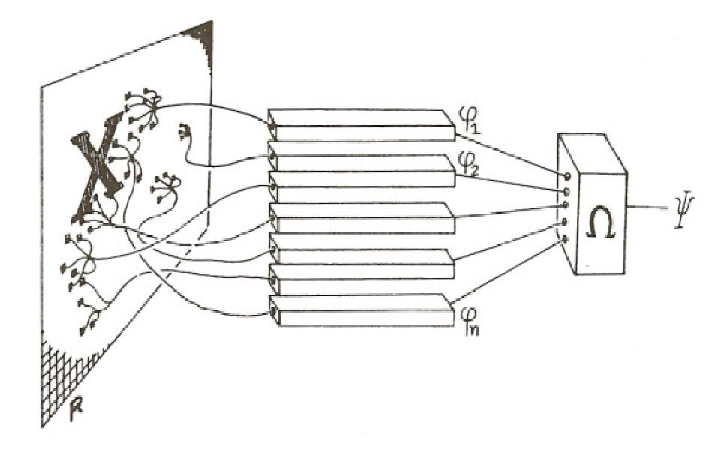
\includegraphics[width=1.0\linewidth]{img/single_layer_cnn.png}
			\caption{Rede neural de arquitetura tipo \textit{feed-forward neural network}.}
			\label{fig:single_layer_cnn.png}
		\end{figure}

		Inicialmente utilizava algoritmos de \textit{backpropagation}, onde cada neurônio propagava seu resultado à todos os neurônios da camada adiante, como exibido na Figura \ref{fig:ffnn.jpg}. Sabendo que a ativação de determinado neurônio dar-se pelo processo de somatório de pesos, esta arquitetura de \textit{feed-forward neural network} (FFNN) não é prática para vários tipos de problemas reais da computação. Um exemplo é a baixa habilidade de reconhecimento de objetos em visualizações. Isso deve-se ao fato de que cada unidade da camada $ n-1 $ é conectada em todas as outras da camada $ n $ na sua propagação. Dessa forma, os números de neurônios e seus cálculos podem crescer exponencialmente com facilidade em relação à sua entrada \cite{Glorot2010}.

		\begin{figure}[H]
			\centering
			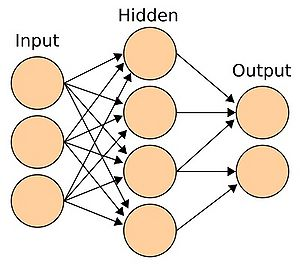
\includegraphics[width=0.8\linewidth]{img/ffnn.jpg}
			\caption{Rede neural FFNN simples.}
			\label{fig:ffnn.jpg}
		\end{figure}

		Para contornar este problema foi necessário uma nova arquitetura que explorasse as restrições espaciais bidimensionais impostas pela sua modalidade de entrada onde reduz simultaneamente a quantidade de parâmetros na sua formação. O nome desta é \textit{convolutional neural network}.


	\subsection{Proposta da Arquitetura \textit{Convolutional Neural Network}}
		Como proposta ao problema do \textit{feed-forward neural network} tem-se a arquitetura \textit{Convolutional Neural Network}. É biologicamente inspirada em variantes de \textit{Multilayer Perceptron} Convolutional Neural Networks (CNN) are biologically-inspired variants of MLPs.

		Ela explora a correlação espacial reforçando um padrão de conectividade local entre neurônios nas camadas adjacentes, ou seja, as entradas da camada $ m $ são de um conjunto da camada anterior $ m-1 $ relacionados de uma forma contígua como é exibido na Figura \ref{fig:layers_cnn} \cite{LeCun1998}.


		\begin{figure}[H]
			\centering
			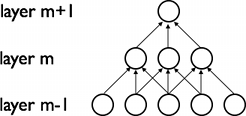
\includegraphics[width=0.8\linewidth]{img/layers_cnn.png}
			\caption{Exemplo das camadas de uma rede \textit{convolutional neural network}.}
			\label{fig:layers_cnn}
		\end{figure}

		O algoritmo baseia-se em vários pequenos processos. São eles a \textit{Convolution}, \textit{Subsampling} e a mescla dos dois processos formando o maior.

		O processo de \textit{Convolução} trata-se da prática de aplicar repetidas vezes a saída de determinada função como entrada de outra. Um termo comumente utilizado para tal processo é também \textit{filtro}, onde a entrada passa por avaliações antes de entrar na segunda e consecutivamente. Já o processo de \textit{Subsampling} utiliza o conhecido algoritmo de \textit{max\_pooling} para reduzir o tamanho de amostras a ser processada pela rede que fará a avaliação booleana da objeto a ser reconhecido \cite{Giusti2013}.

		Tais processos serão praticados na Seção \ref{sec:cnn}.


\section{Desenvolvimento} \label{sec:desenvolvimento}

	\subsection{Procedimentos de Operação de uma \textit{Convolutional Neural Network}} \label{sec:cnn}

		\textit{Neural Networks} podem resolver problemas computacionais complexos utilizando um conjunto simples de neurônios como por exemplo a estimação de preço de uma casa como
		e exibido na Figura \ref{fig:simple_neural}.

		\begin{figure}[H]
			\centering
			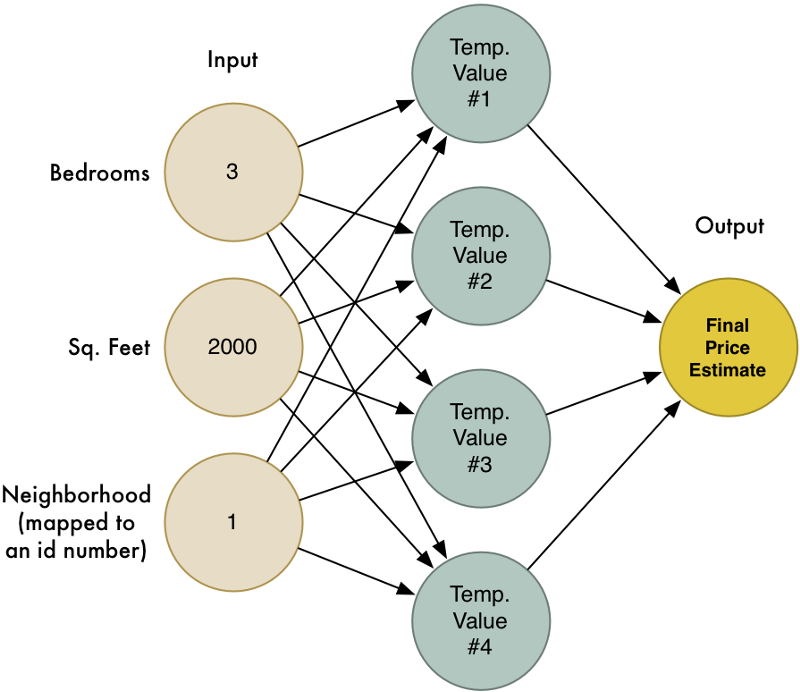
\includegraphics[width=1.0\linewidth]{img/simple_neural.png}
			\caption{Rede neural simples para um problema computacional complexo. Exemplo de um estimador de preço de casa.}
			\label{fig:simple_neural}
		\end{figure}

		São algoritmos genéricos, então alterado este acima, é possível que reconheçamos o número 8 à mão.

		Para que possamos reconhecer determinado item, temos que ter uma prévia de dados para ensinar o algoritmo. Quanto mais dados sobre determinado item, como é mostrado na Figura \ref{fig:entrada_padrao_8}, que no caso é o 8 à mão, melhor será sua acurácia.

		\begin{figure*}[t]
			\centering
			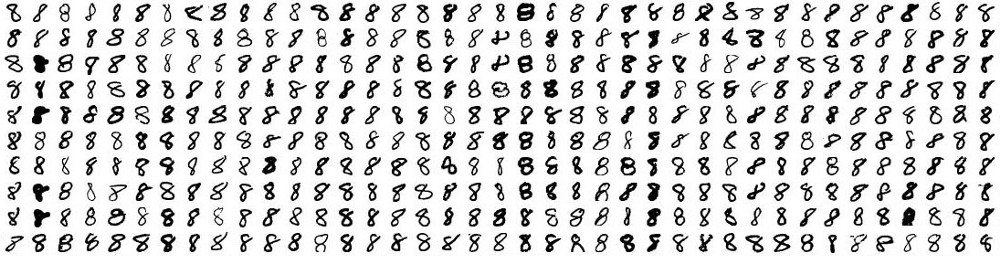
\includegraphics[width=1.0\linewidth]{img/entrada_padrao_8.jpeg}
			\caption{Exemplo de treinamento do algoritmo utilizando vários formatos de 8 escritos à mão livre.}
			\label{fig:entrada_padrao_8}
		\end{figure*}

		Diferente do exemplo do preço que possui somente três entradas, agora temos inúmeras possíveis entradas/escritas do valor 8. As imagens da escrita são digitalizadas e então viram uma entrada para o nosso algoritmo. Usando um padrão de entrada sendo uma imagem 18x18, temos um total de 324 pixels e dessa forma, nosso algoritmo passa de 3 para 324 entradas. Ao contrário da primeira, agora tem-se duas saídas onde cada uma representa a validação do processamento realizado. Um visão geral é exibida na Figura \ref{fig:visao_geral_8}.

		\begin{figure}[H]
			\centering
			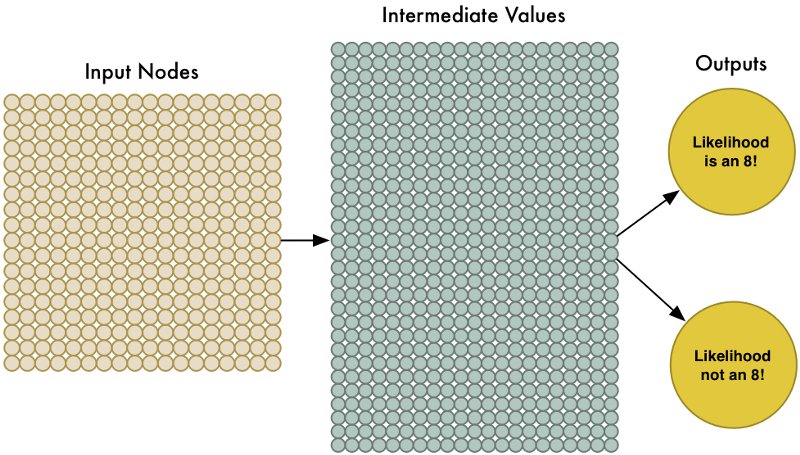
\includegraphics[width=1.0\linewidth]{img/visao_gera_8.png}
			\caption{Visão geral do sistema descrito.}
			\label{fig:visao_geral_8}
		\end{figure}

		Por mais que agora tenhamos centenas de neurônios em nossa rede, computadores modernos ainda conseguem trabalhar e com bom desempenho. Isso é importante pois significa que pode-se executar tais procedimentos em sistemas embutidos onde têm como requisito a economia de energia e processamento mais brandos.

		Após estes passos, deve-se treinar o algoritmo tanto para imagens que representam o valor 8 tanto para as que não representam. Com o algoritmo treinado, temos então uma rede neural capaz de reconhecer valores de 8 escritos à mão com alto valor de acurácia.


		\subsubsection{Enquadramento da Imagem}
			Antes do algoritmo de executar, é necessário enquadrar o que se quer pesquisar para enviar-se como entrada ao algoritmo. Para isso existe algumas técnicas:

			\paragraph{Busca utilizando Janela Deslizante}
				Neste algoritmo, existe uma máscara que percorre toda a imagem. A cada iteração, a máscara seleciona parte da imagem e realiza a pesquisa na rede neural. Realizada a operação em determinado ponto, a máscara realiza o deslizamento para um outro ponto próximo predefinido para a realização de uma nova pesquisa;


			\paragraph{Utilização de dados mais variantes}
				Sabendo-se que a imagem a ser testada pode estar com com uma posição diferente, tamanho ou até mesmo rotação diferente da treinada no algoritmo, permite-se então a criação de outra técnica que procura mais dados com posições variantes para que a rede também possa captar tais tipos de entradas em momentos futuros.

				Entretanto, esta técnica faz com que o algoritmo tenha mais camadas e consequentemente mais complexo\footnote{Técnica ideal para utilização de GPUs.}.

				Ambos, \textit{a)} e \textit{b)} possuem um procedimento custoso, pois utiliza-se técnica de força bruta para a sua pesquisa.


			\paragraph{Convolução}
				Ao invés de usar uma imagem inteira como alimento para a rede neural, utiliza técnicas mais elaboradas para extrair uma vantagem maior.

				Primeiro quebra-se a imagem em vários quadros\footnote{Semelhante a ideia de Janelas Deslizantes.} sendo o nome deste é \textit{Convolução}. Feito isso, utiliza-se cada quadro em uma pequena rede neural. Os resultados serão salvos numa matriz que segue a indexação da imagem original. A matriz de resultados final será avaliada com algoritmo de \texttt{max\_pooling} onde selecionará o melhor resultado em determinado quadrante resultando em uma matriz só de soluções válidas e este processo chama-se \textit{Redução de Amostragem}.

				A função \texttt{max\_pooling} é uma forma de sub-amostragem não-linear. Ela particiona a imagem de entrada em um conjunto não sobreposto de retângulos e para cada tipo de sub-região, retorna o máximo valor encontrado. Seu propósito é a eliminação de valores não maximais reduzindo o processamento computacional nas camadas posteriores. Ela também provê uma forma de transação invariante no processo realizado. Isso provê uma robustez adicional na posição, ela também é uma forma inteligente de reduzir a dimensionalidade de representações intermediárias do processo.

				Com esse processo, elimina-se os itens irrelevantes para o processamento. O processo é demonstrado na Figura \ref{fig:max_pooling.png}.

				\begin{figure}[H]
					\centering
					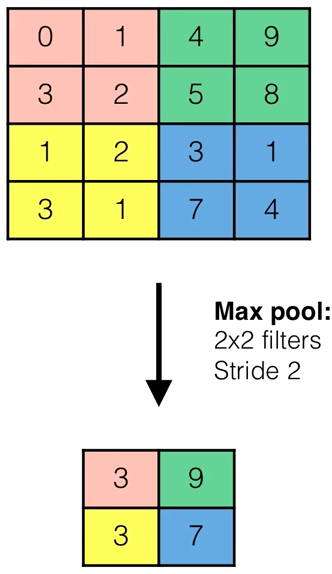
\includegraphics[width=0.5\linewidth]{img/max_pooling.png}
					\caption{O processo de seleção de melhores resultados. Procedimento executado pela função \texttt{max\_pooling}.}
					\label{fig:max_pooling.png}
				\end{figure}

				Os itens resultantes serão entrada para outra rede neural que fará de fato a decisão final de casamento. Tal teoria é exibida na Figura \ref{fig:convolucao_teoria}.

				\begin{figure*}[h]
					\centering
					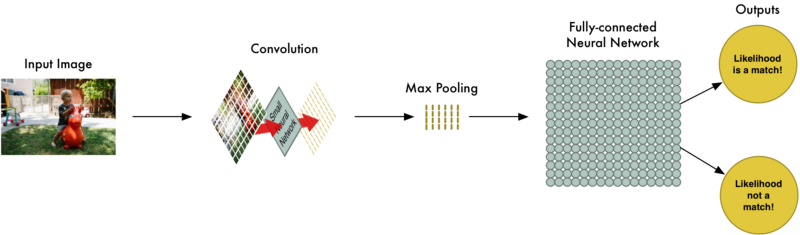
\includegraphics[width=1.0\linewidth]{img/convolucao_teoria.png}
					\caption{O processo simples de uma arquitetura de reconhecimento de padrão \textit{convolutional neural network} final após todos os processos.}
					\label{fig:convolucao_teoria}
				\end{figure*}

				Com tais procedimentos, conclui-se o processo de avaliação utilizando \textit{convolutional neural network}.


		\subsection{Data Set}
			Para testes do algoritmo a ser implementado, será utilizado o conjunto de dados e \textit{benchmark} disponibilizado gratuitamente pela Universidade de Massachusets Amherst \cite{fddbTech}.

			Tal \textit{data-set} possui um conjunto de anotações para 5171 faces identificadas num conjunto de 2845 imagens retiras do conjunto nomeado \textit{Faces in the Wild}, disponível em \url{http://tamaraberg.com/faceDataset/index.html}. O conjunto inteiro possui um total de 30281 imagens com faces coletadas da fonte \textit{News Photographs}. Todas foram automaticamente etiquetadas por meio do sistema descritivo \textit{Who's in the Picture}, no qual possui 80\% de acurácia \cite{berg2004s}.

			Os dados estão em formato compactado \texttt{jpg}. Junto com o pacote de imagens, existe um arquivo com o seguinte formato:

			\begin{verbatim}
				...
				<image name i>
				<number of faces in this image =im>
				<face i1>
				<face i2>
				...
				<face im>
				...
			\end{verbatim}

			onde cada face é denotada por

			\begin{verbatim}
				<major_axis_radius minor_axis_radius angle
				 center_x center_y 1>
			\end{verbatim}

			no qual tais valores representam a posição da face como é exibido na Figura \ref{fig:mulher}.

			\begin{figure}[H]
				\centering
				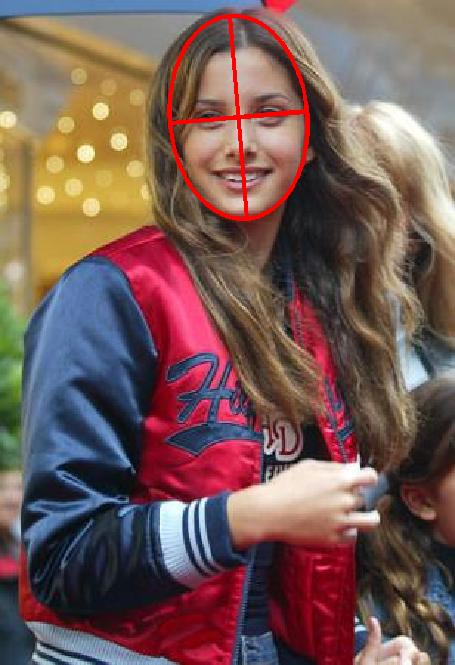
\includegraphics[width=0.75\linewidth]{img/data_set.jpg}
				\caption{Exemplo de identificação de rosto especificado pelo \textit{data-set} disponibilizado pela Universidade de Massachusets Amherst.}
				\label{fig:mulher}
			\end{figure}

%==========================================
\iffinal

\fi



%==========================================

% trigger a \newpage just before the given reference
% number - used to balance the columns on the last page
% adjust value as needed - may need to be readjusted if
% the document is modified later
%\IEEEtriggeratref{8}
% The "triggered" command can be changed if desired:
%\IEEEtriggercmd{\enlargethispage{-5in}}

\bibliographystyle{IEEEtran}
\bibliography{bib_extra/IEEEabrv,example}

%\begin{thebibliography}{1}

%\bibitem{sibgrapi2013}
%\emph{Sibgrapi 2013, Proceedings of the XXVI Brazilian Symposium on Computer Graphics and Image Processing}.\hskip 1em plus 0.5em minus 0.4em\relax  Arequipa, Per{\'u}: {IEEE}, august 2013.

%\end{thebibliography}




\end{document}

%==========================================
